% !TeX spellcheck = en_GB

\section{Requirements}\label{sec:requirements}

The following sections describe the primary requirements in the form of user stories~\cite{agile-alliance-user-stories}.
Figure~\ref{fig:requirements-overview} shows an overview of the primary use stories.

\begin{figure}[h]
    \centering
    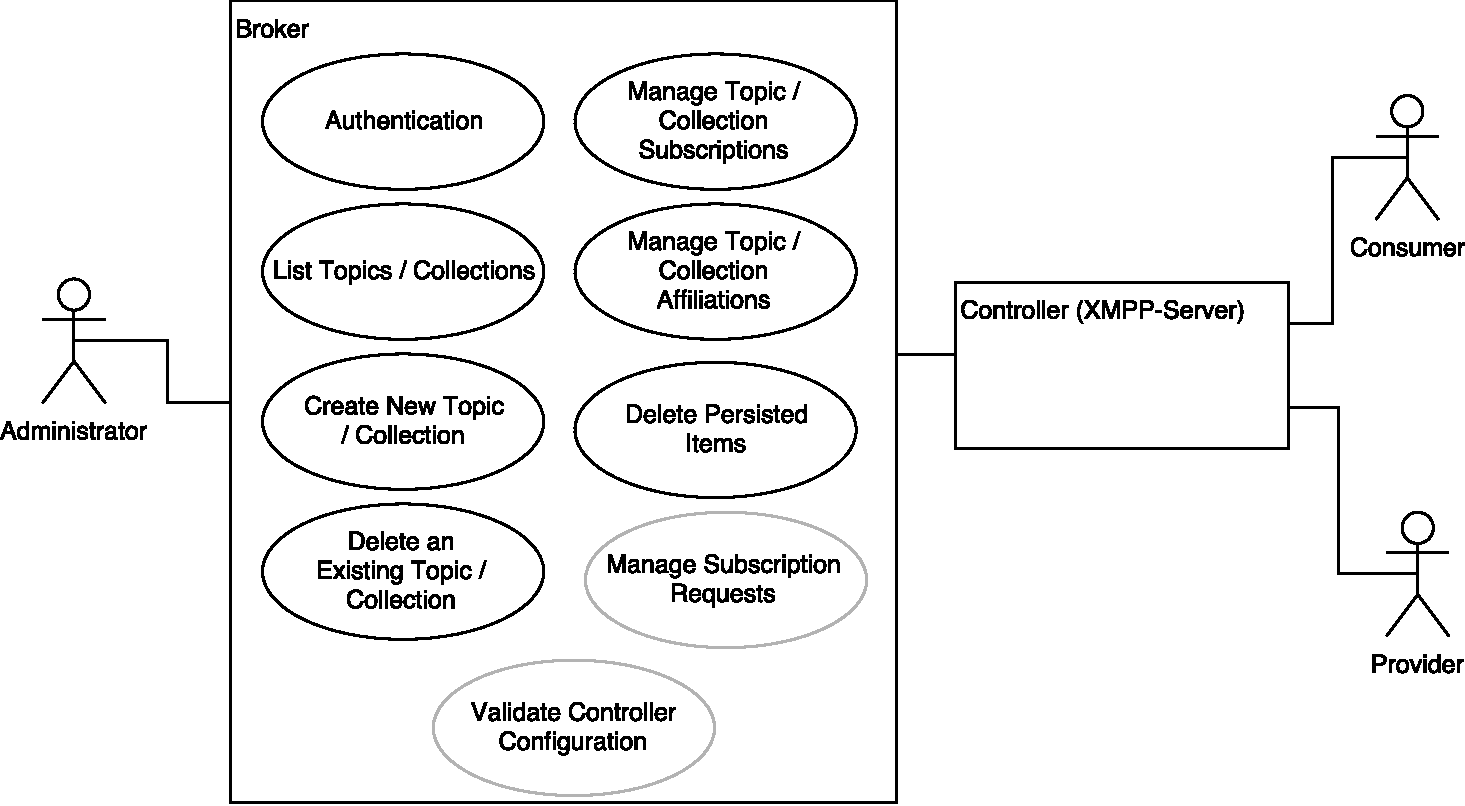
\includegraphics[width=1\linewidth]{resources/requirements_overview}
    \caption{UML Use Case Diagram presenting an overview of the primary user stories.}
    \label{fig:requirements-overview}
\end{figure}

\subsection{Authentication}\label{sec:authentication}
\subsubsection{Login}

As an Administrator,\\
I want to log in\\
- preferably using an existing client TLS certificate - \\
so that only I can inspect and manage Topics.\\

\subsubsection{Secure \gls{xmpp} Authentication}

As an Administrator concerned with security requirements,\\
I want to use either \gls{sasl-external} or \gls{sasl-scram} mechanism for authentication -

\begin{itemize}
    \item preferably the SCRAM-SHA-256-PLUS variant and
    \item preferably using mutual certificate-based authentication including revocation status checking
\end{itemize}

\noindent - so that the Controller is fully compatible with the \gls{xmpp-grid} standard~\cite{ietf-mile-xmpp-grid-05}.

\noindent To achieve this goal, I am willing to accept:
\begin{itemize}
    \item More costly and less user friendly authentication
    \item limited compatibility of supported \gls{xmpp} servers
\end{itemize}

\subsubsection{Secure \gls{xmpp} Connection}

As an Administrator concerned with security requirements,\\
I want to use minimally TLS 1.2 [RFC5246] to communicate with the \gls{xmpp} server at all times\\
to achieve maximal security and compatibility with the \gls{xmpp-grid} standard~\cite{ietf-mile-xmpp-grid-05}.

\subsubsection{Secure Connection}

As an Administrator concerned with security requirements,\\
I want to use minimally TLS 1.2 [RFC5246] to communicate with the Broker\\
to achieve maximal security.

\subsubsection{Multiple Administrators}\label{sec:requirement-multiple-administrators}

As an Administrator,\\
I want to grant access to administrators \\
so that they can also manage the application.

\subsubsection{Audit Trail}\label{sec:requirement-audit-trail}

As an Administrator concerned with security requirements,\\
I want to be able to access an audit log\\
- preferably using existing \gls{xmpp} mechanisms - \\
so that I can reconstruct what other Administrations did on the Controller.

\subsubsection{Logout}\label{sec:requirement-logout}

As an Administrator,\\
I want to log out\\
so that I can terminate a session.

\subsection{List Topics and Collections}\label{sec:list-topics}

\subsubsection{List All Topics}\label{sec:requirement-list-all-topics}
As an Administrator,\\
I want to see a list of all Topics of the associated Controller\\
so that I can quickly assimilate which Topics exist.

\subsubsection{List All Top-Level-Collections}
As an Administrator,\\
I want to see a list of all Top-Level-Collections of the associated Controller\\
so that I can quickly assimilate which Collections exist.

\subsubsection{List All Parent-Collections of a Topic}
As an Administrator,\\
I want to see a list of all transitive parent Collections that contain a given Topic\\
so that I can quickly assimilate in which Collections items are published.

\subsubsection{List All Subtopics and Subcollection of a Collection}
As an Administrator,\\
I want to see a list of all Collections and Topics that a given Collection contains\\
so that I can quickly assimilate the collection hierarchy.

\subsubsection{List Available Topics With Limited Access (optional)}

As an Administrator,\\
I want to see a list of all Topics of the associated Controller to which I have limited access to,\\
to simplify troubleshooting and locate errors.

\subsubsection{List Available Collections With Limited Access (optional)}

As an Administrator,\\
I want to see a list of all Collections of the associated Controller to which I have limited access to,\\
to simplify troubleshooting and locate errors.

\subsubsection{Topic and Collection Paging}
As an Administrator,\\
I want to be able to page through any set of Collection/Topic with more than 10 Items \\
so that I can work with more than 1000 Collections and Topics more effectively.

\subsubsection{Topic and Collection Name Filter}\label{sec:requirement-topic-filter}
As an Administrator,\\
I want to be able to quickly filter any set of Collections/Topics with more than 10 Items \\
so that I can work with more than 1000 Collections and Topics more effectively.

\subsection{Create a New Topic}\label{sec:create-topic}

As an Administrator,\\
I want to create a new Topic on the associated Controller\\
so that I am not tied to a fixed set of Topics.

\subsection{Create a New Collection}\label{sec:create-collection}

As an Administrator,\\
I want to create a new Collection on the associated Controller\\
so that I can flexibly patch Topics together.

\subsubsection{Override Default Topic Configuration}\label{sec:requirement-topic-default-configuration}

As an Administrator in the process of creating a new Topic,\\
I want to override the default configuration (e.g. the affiliations) \\
so that I can restrict access and provide reasonable defaults.

\subsubsection{Override Default Collection Configuration}\label{sec:requirement-collection-default-configuration}

As an Administrator in the process of creating a new Collection,\\
I want to override the default configuration (e.g. the affiliations) \\
so that I can restrict access and provide reasonable defaults.

\subsubsection{Initial Topic Consumers and Providers}\label{sec:requirement-initial-topic-consumer-provider}

As an Administrator in the process of creating a new Topic,\\
I want to specify an initial set of Consumers and Providers \\
so that I can restrict access to that Topic and provide reasonable defaults.

\subsubsection{Initial Collection Consumers}\label{sec:requirement-initial-collection-consumer}

As an Administrator in the process of creating a new Collection,\\
I want to specify an initial set of Consumers \\
so that I can restrict access to that Collection and provide reasonable defaults.

\subsection{Delete an Existing Topic}\label{sec:delete-topic}

As an Administrator,\\
I want to delete an existing Topic on the associated Controller\\
so that I can get rid of obsolete Topics.

\subsection{Delete an Existing Collection}\label{sec:delete-collection}

As an Administrator,\\
I want to delete an existing Collection on the associated Controller\\
so that I can get rid of obsolete Collections.


\subsubsection{Fault Prevention On Topic-Delete}

As an Administrator in the process of deleting a Topic, \\
I want a mechanism to prevent me from deleting the wrong Topic on the associated Controller\\
(e.g. require me to enter the name of the Topic manually).

\subsubsection{Fault Prevention On Collection-Delete}

As an Administrator in the process of deleting a Collection, \\
I want a mechanism to prevent me from deleting the wrong Collection on the associated Controller\\
(e.g. require me to enter the name of the Collection manually).


\subsection{Manage Topic/Collection Subscriptions}\label{sec:manage-subscriptions}

\subsubsection{List Consumers}

As an Administrator, \\
I want to list all Consumers (including their JIDs) of a given Topic/Collection on the associated Controller, \\
so that I can verify that specific Consumers are subscribed, and others are not.


\subsubsection{Inspect Detailed Subscription Configuration}

As an Administrator, \\
I want to inspect the detailed Topic/Collection subscription configuration of a given Consumer, \\
so that I can reproduce and reason about the receipt of data on that Consumer
and find potential misconfiguration.

\subsubsection{Partially Modify Subscription Configuration}

As an Administrator, \\
I want to modify parts of the Topic/Collection subscription configuration of a given Consumer, \\
so that I can fix misconfiguration.

\subsubsection{Unsubscribe Consumer}

As an Administrator, \\
I want to manually unsubscribe a specific Consumer from a particular Topic/Collection on the associated Controller, \\
so that I can remove obsolete or undesired subscriptions.

\subsubsection{Subscribe Consumer}

As an Administrator, \\
I want to manually subscribe a specific Consumer on a particular Topic/Collection on the associated Controller, \\
so that I can faster setup and manage Consumers.

\subsection{Manage Topic Affiliations}\label{sec:manage-affiliations}
\subsubsection{Inspect Affiliations}

As an Administrator,\\
I want to list all Affiliations (JID and "Role") for a particular Topic/Collection on the associated Controller \\
so that I can find potential misconfiguration.

\subsubsection{Modify Affiliations}

As an Administrator,\\
I want to modify the Affiliation ("Role") of a given JID for a particular Topic/Collection on the associated Controller \\
so that I can fix potential misconfiguration.

\subsubsection{Fault Prevention When Modifying My Affiliation}

As an Administrator in the process of modifying my Affiliation for a particular Topic/Collection on the associated Controller,\\
I want a mechanism to prevent me from accidentally downgrading my rights.

\subsubsection{Meaningful Error For Topics/Collection With Limited Access}

As an Administrator,\\
I want to receive a meaningful error message when inspecting a Topic/Collection to which I have limited access \\
so that I can quickly comprehend why the configuration options are limited.

\subsection{Manage Persisted Items of a Topic}\label{sec:manage-persisted-items}
\subsubsection{Inspect Persisted Items}

As an Administrator,\\
I want to list all Persisted Items for a particular Topic on the associated Controller \\
so that I can get an overview and check for misconfiguration.

\subsubsection{Filter Persisted Items}\label{sec:requirement-filter-persisted-items}

As an Administrator,\\
I want to be able to filter all persisted Items of a specific Topic by \\
\begin{itemize}
    \item the timestamp of its publication
    \item the publishers JID
\end{itemize}
so that I can work with more than 10000 persisted items more effectively.

\subsubsection{Paged Persisted Items}\label{sec:paged-persisted-items}
As an Administrator working with filtered persisted items,\\
I want to be able to page through the resulting items\\
- given that this feature is supported by the associated Controller -\\
so that I can work with more than 10000 persisted items more effectively.

\subsubsection{Delete a Persisted Item From a Topic}

As an Administrator,\\
I want to delete a particular persisted item from a specific Topic\\
- given that this feature is supported by the associated Controller -\\
so that I can clean up test items and remove obsolete or corrupted items.

\subsubsection{Purge All Persisted Items From a Topic}

As an Administrator,\\
I want to purge persisted items from a specific Topic\\
- given that this feature is supported by the associated Controller -\\
so that I can clean up test items and remove obsolete or corrupted items.

\subsubsection{Delete Set of Persisted Item From a Topic (optional)}

As an Administrator,\\
I want to delete a set of persisted item that match a given criteria from a specific Topic\\
- given that this feature is supported by the associated Controller -\\
so that I can clean up test items and remove obsolete or corrupted items.

\subsection{Manage Subscription Requests (optional)}\label{sec:subscription-requests}

\subsubsection{List Subscription Request}
As an Administrator,\\
I want to list pending subscription requests for a given Topic\\
- given that this feature is supported by the associated Controller -\\
so that I can quickly assimilate pending requests.

\subsubsection{Accept Subscription Request}

As an Administrator,\\
I want to accept a pending subscription request for a given Topic\\
- given that this feature is supported by the associated Controller -\\
to enable more dynamic access models than just maintaining a black- or whitelist.

\subsubsection{Reject Subscription Request}

As an Administrator,\\
I want to reject a pending subscription request for a given Topic\\
- given that this feature is supported by the associated Controller -\\
so that I can deny user access in accordance with the \gls{xmpp} standards.

\subsection{Validate Controller Configuration (optional)}\label{sec:validate-controller-config}

\subsubsection{Validate Supported XEPs Configurations}
As an Administrator,\\
I want to validate that a minimum set of XEPs are supported by the associated Controller\\
so that I can quickly identify incompatibilities.

\subsubsection{Validate Optional XEP Implementations}
As an Administrator,\\
I want to validate that the required features that are marked as optional or recommended in the XEPs are implemented by the associated Controller\\
so that I can quickly identify incompatibilities.

